% Options for packages loaded elsewhere
\PassOptionsToPackage{unicode}{hyperref}
\PassOptionsToPackage{hyphens}{url}
\PassOptionsToPackage{dvipsnames,svgnames,x11names}{xcolor}
%
\documentclass[
]{article}
\usepackage{amsmath,amssymb}
\usepackage{lmodern}
\usepackage{iftex}
\ifPDFTeX
  \usepackage[T1]{fontenc}
  \usepackage[utf8]{inputenc}
  \usepackage{textcomp} % provide euro and other symbols
\else % if luatex or xetex
  \usepackage{unicode-math}
  \defaultfontfeatures{Scale=MatchLowercase}
  \defaultfontfeatures[\rmfamily]{Ligatures=TeX,Scale=1}
\fi
% Use upquote if available, for straight quotes in verbatim environments
\IfFileExists{upquote.sty}{\usepackage{upquote}}{}
\IfFileExists{microtype.sty}{% use microtype if available
  \usepackage[]{microtype}
  \UseMicrotypeSet[protrusion]{basicmath} % disable protrusion for tt fonts
}{}
\makeatletter
\@ifundefined{KOMAClassName}{% if non-KOMA class
  \IfFileExists{parskip.sty}{%
    \usepackage{parskip}
  }{% else
    \setlength{\parindent}{0pt}
    \setlength{\parskip}{6pt plus 2pt minus 1pt}}
}{% if KOMA class
  \KOMAoptions{parskip=half}}
\makeatother
\usepackage{xcolor}
\IfFileExists{xurl.sty}{\usepackage{xurl}}{} % add URL line breaks if available
\IfFileExists{bookmark.sty}{\usepackage{bookmark}}{\usepackage{hyperref}}
\hypersetup{
  pdftitle={Foundations of community ecology},
  colorlinks=true,
  linkcolor={blue},
  filecolor={Maroon},
  citecolor={Blue},
  urlcolor={Blue},
  pdfcreator={LaTeX via pandoc}}
\urlstyle{same} % disable monospaced font for URLs
\usepackage[margin=1in]{geometry}
\usepackage{color}
\usepackage{fancyvrb}
\newcommand{\VerbBar}{|}
\newcommand{\VERB}{\Verb[commandchars=\\\{\}]}
\DefineVerbatimEnvironment{Highlighting}{Verbatim}{commandchars=\\\{\}}
% Add ',fontsize=\small' for more characters per line
\usepackage{framed}
\definecolor{shadecolor}{RGB}{248,248,248}
\newenvironment{Shaded}{\begin{snugshade}}{\end{snugshade}}
\newcommand{\AlertTok}[1]{\textcolor[rgb]{0.94,0.16,0.16}{#1}}
\newcommand{\AnnotationTok}[1]{\textcolor[rgb]{0.56,0.35,0.01}{\textbf{\textit{#1}}}}
\newcommand{\AttributeTok}[1]{\textcolor[rgb]{0.77,0.63,0.00}{#1}}
\newcommand{\BaseNTok}[1]{\textcolor[rgb]{0.00,0.00,0.81}{#1}}
\newcommand{\BuiltInTok}[1]{#1}
\newcommand{\CharTok}[1]{\textcolor[rgb]{0.31,0.60,0.02}{#1}}
\newcommand{\CommentTok}[1]{\textcolor[rgb]{0.56,0.35,0.01}{\textit{#1}}}
\newcommand{\CommentVarTok}[1]{\textcolor[rgb]{0.56,0.35,0.01}{\textbf{\textit{#1}}}}
\newcommand{\ConstantTok}[1]{\textcolor[rgb]{0.00,0.00,0.00}{#1}}
\newcommand{\ControlFlowTok}[1]{\textcolor[rgb]{0.13,0.29,0.53}{\textbf{#1}}}
\newcommand{\DataTypeTok}[1]{\textcolor[rgb]{0.13,0.29,0.53}{#1}}
\newcommand{\DecValTok}[1]{\textcolor[rgb]{0.00,0.00,0.81}{#1}}
\newcommand{\DocumentationTok}[1]{\textcolor[rgb]{0.56,0.35,0.01}{\textbf{\textit{#1}}}}
\newcommand{\ErrorTok}[1]{\textcolor[rgb]{0.64,0.00,0.00}{\textbf{#1}}}
\newcommand{\ExtensionTok}[1]{#1}
\newcommand{\FloatTok}[1]{\textcolor[rgb]{0.00,0.00,0.81}{#1}}
\newcommand{\FunctionTok}[1]{\textcolor[rgb]{0.00,0.00,0.00}{#1}}
\newcommand{\ImportTok}[1]{#1}
\newcommand{\InformationTok}[1]{\textcolor[rgb]{0.56,0.35,0.01}{\textbf{\textit{#1}}}}
\newcommand{\KeywordTok}[1]{\textcolor[rgb]{0.13,0.29,0.53}{\textbf{#1}}}
\newcommand{\NormalTok}[1]{#1}
\newcommand{\OperatorTok}[1]{\textcolor[rgb]{0.81,0.36,0.00}{\textbf{#1}}}
\newcommand{\OtherTok}[1]{\textcolor[rgb]{0.56,0.35,0.01}{#1}}
\newcommand{\PreprocessorTok}[1]{\textcolor[rgb]{0.56,0.35,0.01}{\textit{#1}}}
\newcommand{\RegionMarkerTok}[1]{#1}
\newcommand{\SpecialCharTok}[1]{\textcolor[rgb]{0.00,0.00,0.00}{#1}}
\newcommand{\SpecialStringTok}[1]{\textcolor[rgb]{0.31,0.60,0.02}{#1}}
\newcommand{\StringTok}[1]{\textcolor[rgb]{0.31,0.60,0.02}{#1}}
\newcommand{\VariableTok}[1]{\textcolor[rgb]{0.00,0.00,0.00}{#1}}
\newcommand{\VerbatimStringTok}[1]{\textcolor[rgb]{0.31,0.60,0.02}{#1}}
\newcommand{\WarningTok}[1]{\textcolor[rgb]{0.56,0.35,0.01}{\textbf{\textit{#1}}}}
\usepackage{graphicx}
\makeatletter
\def\maxwidth{\ifdim\Gin@nat@width>\linewidth\linewidth\else\Gin@nat@width\fi}
\def\maxheight{\ifdim\Gin@nat@height>\textheight\textheight\else\Gin@nat@height\fi}
\makeatother
% Scale images if necessary, so that they will not overflow the page
% margins by default, and it is still possible to overwrite the defaults
% using explicit options in \includegraphics[width, height, ...]{}
\setkeys{Gin}{width=\maxwidth,height=\maxheight,keepaspectratio}
% Set default figure placement to htbp
\makeatletter
\def\fps@figure{htbp}
\makeatother
\setlength{\emergencystretch}{3em} % prevent overfull lines
\providecommand{\tightlist}{%
  \setlength{\itemsep}{0pt}\setlength{\parskip}{0pt}}
\setcounter{secnumdepth}{-\maxdimen} % remove section numbering
\newlength{\cslhangindent}
\setlength{\cslhangindent}{1.5em}
\newlength{\csllabelwidth}
\setlength{\csllabelwidth}{3em}
\newlength{\cslentryspacingunit} % times entry-spacing
\setlength{\cslentryspacingunit}{\parskip}
\newenvironment{CSLReferences}[2] % #1 hanging-ident, #2 entry spacing
 {% don't indent paragraphs
  \setlength{\parindent}{0pt}
  % turn on hanging indent if param 1 is 1
  \ifodd #1
  \let\oldpar\par
  \def\par{\hangindent=\cslhangindent\oldpar}
  \fi
  % set entry spacing
  \setlength{\parskip}{#2\cslentryspacingunit}
 }%
 {}
\usepackage{calc}
\newcommand{\CSLBlock}[1]{#1\hfill\break}
\newcommand{\CSLLeftMargin}[1]{\parbox[t]{\csllabelwidth}{#1}}
\newcommand{\CSLRightInline}[1]{\parbox[t]{\linewidth - \csllabelwidth}{#1}\break}
\newcommand{\CSLIndent}[1]{\hspace{\cslhangindent}#1}
\usepackage{fancyhdr}
\ifLuaTeX
  \usepackage{selnolig}  % disable illegal ligatures
\fi

\title{Foundations of community ecology}
\author{A. Bradley Duthie\(^{1,a,*}\) and Victor J. Luque\(^{2,a}\)}
\date{{[}1{]} Department of Biological and Environmental Sciences,
University of Stirling, Stirling, Scotland {[}2{]} Department of
Philosophy, University of Valencia, Valencia, Spain {[}*{]}
Corresponding author:
\href{mailto:alexander.duthie@stir.ac.uk}{\nolinkurl{alexander.duthie@stir.ac.uk}}
{[}a{]} Equal contribution}

\begin{document}
\maketitle

We have discovered the fundamental equation that provides a complete
description of eco-evolutionary change in any system,

\[\Omega = \sum_{i=1}^{N} \left(\beta_{i} - \delta_{i} + 1 \right)\left(z_{i} + \Delta z_{i} \right).
\tag{1}
\]

In our previous efforts, we derived both the Price equation and the
birth-death model from the above. Here we can derive a fundamental model
of community ecology, a discrete time generalised Lotka-Volterra
equations leading to modern coexistence theory. We can do this by
partitioning the sum total change \(\Omega\) into change caused by
density-independent and density-dependent effects,

\[\Omega = \sum_{i=1}^{N} \left(\beta_{i} - \delta_{i} + 1 \right)\left(z_{i} + \Delta z_{i} \right)\left(1 - \sum_{j = 1}^{N}\left(a_{ij}\left(z_{i} + \Delta z_{i} \right) \right) \right).
\tag{2}
\]

In eqn 2, \(a_{ij}\) is the effect that \(j\) has on the contribution of
\(i\) to \(\Omega\). Note that we are, again, not relaxing an assumption
in eqn 1, nor are we adding something that did not already exist to the
model. Equation 1 is already a complete description of eco-evolutionary
change, so it included both density-independent and density-dependent
effects. The new expression in parentheses is only splitting the total
change into density-independent versus density-dependent effects. As
with the previous case of ecology, we can set \(z_{i} = 1\) and
\(\Delta z_{i} = 0\), which allows us to simplify,

\[\Omega = \sum_{i=1}^{N} \left(\beta_{i} - \delta_{i} + 1 \right)\left(1 - \sum_{j = 1}^{N}a_{ij} \right).
\tag{3}
\]

Now, assume that every individual \(j\) in the population has an
identical effect on \(i\), such that \(a_{ij} = \alpha\). With the
conceptual understanding that \(\alpha\) is then the per capita effect
of \(j\) on \(i\), we can rewrite eqn 3,

\[\Omega = \sum_{i=1}^{N} \left(\beta_{i} - \delta_{i} + 1 \right)\left(1 - \sum_{j = 1}^{N}\alpha \right).
\]

Because we then sum up \(\alpha\) a total of \(N\) times, it then
follows,

\[\Omega = \sum_{i=1}^{N} \left(\beta_{i} - \delta_{i} + 1 \right)\left(1 - \alpha N \right).
\]

Now, we can again assume that individual births (\(b = \beta_{i}\)) and
deaths (\(d = \delta_{i}\)) are identical for all \(i\),

\[\Omega = \sum_{i=1}^{N} \left(b -d + 1 \right)\left(1 - \alpha N \right).
\]

Because we define \(\lambda = b - d + 1\),

\[\Omega = \sum_{i=1}^{N} \lambda\left(1 - \alpha N \right).
\]

We now have removed all subscripts \(i\) from the right-hand side, and
we can rewrite,

\[\Omega =  N \lambda\left(1 - \alpha N \right).
\]

Now is a good time to define \(\Omega\) again and add subscripts to
\(N\),

\[N_{t+1} =  N_{t} \lambda\left(1 - \alpha N_{t} \right).
\tag{4}
\]

Equation 4 gives us a discrete time logistic growth equation. This is
not typically the way a discrete time equation is expressed, which made
me a bit nervous at first, but there is nothing wrong with it either.

We can do some simple simulations to confirm that it behaves as it
should. I am going to make a lot of common simplifying assumptions in
what follows (rather, I already have in eqn 4). I assume that \(\alpha\)
and \(\lambda\) are constant and do not change with density. Suppose
then that we have a population of just two individuals, \(N_{t} = 2\).
With density independent effects, assume that the population is doubling
from \(t\) to \(t + 1\), so \(\lambda = 2\). Now assume that the effect
of each individual in the population is to decrease each other
individual's growth by \(\alpha = 0.01\). We then have
\(N_{t+1} = 2 N_{t} \left(1 - 0.01 N_{t} \right)\). We can simulate this
over 10 time steps.

\begin{Shaded}
\begin{Highlighting}[]
\NormalTok{NN }\OtherTok{\textless{}{-}} \DecValTok{2}\NormalTok{;}
\NormalTok{LL }\OtherTok{\textless{}{-}} \DecValTok{2}\NormalTok{;}
\NormalTok{aa }\OtherTok{\textless{}{-}} \FloatTok{0.01}\NormalTok{;}
\NormalTok{tt }\OtherTok{\textless{}{-}} \DecValTok{10}\NormalTok{;}
\NormalTok{i  }\OtherTok{\textless{}{-}} \DecValTok{1}\NormalTok{;}
\ControlFlowTok{while}\NormalTok{(i }\SpecialCharTok{\textless{}}\NormalTok{ tt)\{}
\NormalTok{    Nt        }\OtherTok{\textless{}{-}}\NormalTok{ NN[i]}\SpecialCharTok{*}\NormalTok{LL}\SpecialCharTok{*}\NormalTok{(}\DecValTok{1} \SpecialCharTok{{-}}\NormalTok{ aa }\SpecialCharTok{*}\NormalTok{ NN[i]);}
\NormalTok{    NN[i }\SpecialCharTok{+} \DecValTok{1}\NormalTok{] }\OtherTok{\textless{}{-}}\NormalTok{ Nt;}
\NormalTok{    i         }\OtherTok{\textless{}{-}}\NormalTok{ i }\SpecialCharTok{+} \DecValTok{1}\NormalTok{;}
\NormalTok{\}}
\FunctionTok{print}\NormalTok{(NN);}
\end{Highlighting}
\end{Shaded}

\begin{verbatim}
##  [1]  2.000000  3.920000  7.532672 13.930521 23.979854 36.459040 46.332848
##  [8] 49.731040 49.998553 50.000000
\end{verbatim}

\begin{Shaded}
\begin{Highlighting}[]
\FunctionTok{plot}\NormalTok{(}\AttributeTok{x =} \DecValTok{1}\SpecialCharTok{:}\DecValTok{10}\NormalTok{, }\AttributeTok{y =}\NormalTok{ NN, }\AttributeTok{type =} \StringTok{"b"}\NormalTok{, }\AttributeTok{pch =} \DecValTok{20}\NormalTok{, }\AttributeTok{lwd =} \DecValTok{2}\NormalTok{,}
     \AttributeTok{xlab =} \StringTok{"Time step"}\NormalTok{,}
     \AttributeTok{ylab =} \StringTok{"Population density (N)"}\NormalTok{);}
\FunctionTok{points}\NormalTok{(}\AttributeTok{x =} \DecValTok{1}\SpecialCharTok{:}\DecValTok{10}\NormalTok{, }\AttributeTok{y =}\NormalTok{ NN, }\AttributeTok{type =} \StringTok{"l"}\NormalTok{, }\AttributeTok{pch =} \DecValTok{20}\NormalTok{, }\AttributeTok{lwd =} \DecValTok{2}\NormalTok{);}
\end{Highlighting}
\end{Shaded}

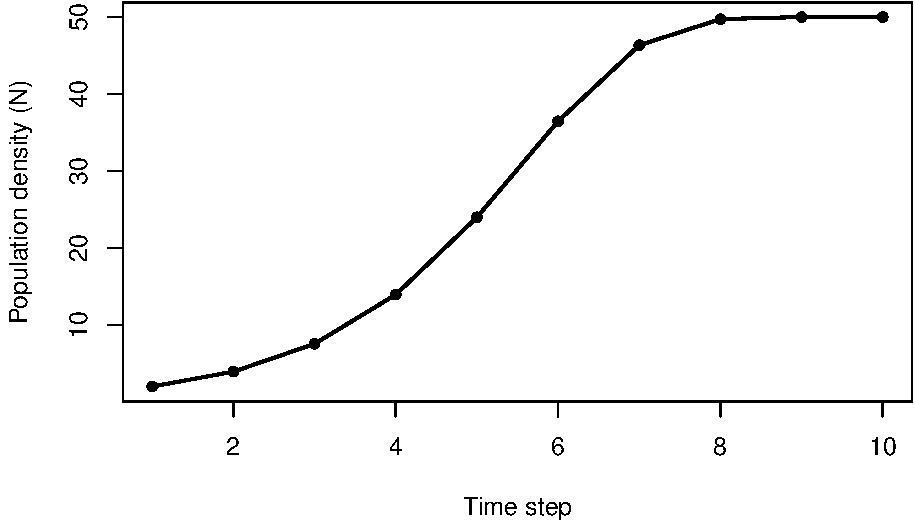
\includegraphics{foundations_of_community_ecology_files/figure-latex/unnamed-chunk-1-1.pdf}

The population increases exponentially, then levels off at \(N = 50\),
at which point the population growth \(N\lambda = 2(50) = 100\) is
balanced by the total effect of competition
\(\alpha N = 50^{2}(2)(0.01) = 50\), such that \(100 - 50\) keeps the
population at \(50\).

I was a bit bothered by the unusual formulation at first, but now I am
feeling better about it. I am convinced it is correct, albeit not the
typically way that researchers tend to model population change. But
usually modellers will switch to continuous time models for logistic
growth and generalised Lotka-Volterra. And for discrete growth, they
will usually do something like
\(N_{t+1} = N_{t} + N_{t}\lambda(1 - N_{t}/K)\), where \(K\) is the
carrying capacity. But this is effort is not derived from first
principles, I do not think, in the same way as the above eqn 4.

\hypertarget{recovering-proper-logistic-growth}{%
\section{Recovering proper logistic
growth}\label{recovering-proper-logistic-growth}}

Note that we can also recover a different logistic growth equation if we
start at eqn 3, but then assume that \(r = b - d\), and density
dependent effects only apply to birth and death,

\[\Omega = \sum_{i=1}^{N} \left(r_{i} + 1 \right)\left(1 - \sum_{j = 1}^{N}a_{ij} \right).
\tag{5}
\]

This seems more reasonable. The effect of an individual \(j\) on a focal
individual \(i\) has to be either on birth or death. The 1 is a
constant, and I do not think it should be affected. Mathematically, we
can expand eqn 5.

\[\Omega = \sum_{i=1}^{N} r_{i}\left(1 - \sum_{j = 1}^{N}a_{ij} \right) + \left(1 - \sum_{j = 1}^{N}a_{ij} \right).\]

Biologically, there is a clear way to resolve this, though I think some
caution is needed here with the mathematics. It is biologically
reasonable that \(a_{ij} = 0\) in the second term for all \(j\). If
\(a_{ij}\) only applies to \(r_{i}\) such that \(a_{ij} = 0\) for all
\(i\) and \(j\) in the second term, then,

\[\Omega = \sum_{i=1}^{N} r_{i}\left(1 - \sum_{j = 1}^{N}a_{ij} \right) + 1.\]

If we can get to this point, then we can make the same assumption that
we did around eqn 3, such that every individual \(j\) has an identical
effect on \(i\), so \(a_{ij} = \alpha\). It then follows,

\[\Omega = \sum_{i=1}^{N} r_{i}\left(1 - \sum_{j = 1}^{N}\alpha \right) + 1.\]

From here, we then sum up the \(\alpha\) values,

\[\Omega = \sum_{i=1}^{N} r_{i}\left(1 - \alpha N \right) + 1.\]

If we assume that \(r_{i} = r\) for all \(i\), then we are also summing
\(r(1 - \alpha N) + 1\) a total of \(N\) times,

\[\Omega = N \left( r_{i}\left(1 - \alpha N \right) + 1\right).\]

By setting \(\Omega = N_{t+1}\) and \(N = N_{t}\), we can then recover,

\[N_{t+1} = N_{t} + rN_{t}\left(1 - \alpha N_{t}\right)\]

Again, in this case, \(\alpha\) reflects interactions among individuals
only affecting birth and death. This is a standard discrete time
generalised Lotka-Volterra equation, as appears in Chesson
(\protect\hyperlink{ref-Chesson2000b}{2000}). To recover community
ecology, it should be a standard matter of defining two sets \(J\) and
\(K\) representing different species,

\[\Omega = \sum_{i=1}^{N} \left(r_{i} + 1 \right)\left(1 - \sum_{j \in J}a_{ij} - \sum_{k \in K}a_{ik} \right).\]

Summations can be made over different scales too, but I think that this
gets us solidly to Chesson (\protect\hyperlink{ref-Chesson2000b}{2000}).

\hypertarget{references}{%
\section*{References}\label{references}}
\addcontentsline{toc}{section}{References}

\hypertarget{refs}{}
\begin{CSLReferences}{1}{0}
\leavevmode\vadjust pre{\hypertarget{ref-Chesson2000b}{}}%
Chesson, Peter L. 2000. {``{Mechanisms of maintenance of species
diversity}.''} \emph{Annual Review of Ecology and Systematics} 31:
343--66.

\end{CSLReferences}

\end{document}
